\documentclass[a4paper,12px]{article}
\usepackage{graphicx}
\usepackage[english]{babel}
\usepackage{fancyhdr}
\usepackage{lastpage}
\usepackage{xifthen}
\usepackage[linesnumberedhidden, titlenotnumbered]{algorithm2e}
\usepackage{lipsum}
\usepackage{hyperref}
\usepackage{array}
\usepackage{tabularx}
\usepackage{caption}
\usepackage{amsfonts}
\usepackage{amssymb}
\usepackage{amsmath}
\usepackage{placeins}
\usepackage{enumitem}
\usepackage{parskip}

\usepackage{minted}
\usepackage{listings}
\usepackage{dsfont}
\usepackage{units}

\pagestyle{fancy}
\lhead{
\includegraphics[width=7cm]{logoUvA}}
\rhead{\footnotesize \textsc {Report\\ \opdracht}}
\lfoot
{%
    \footnotesize \studentA
    \ifthenelse{\isundefined{\studentB}}{}{\\ \studentB}
    \ifthenelse{\isundefined{\studentC}}{}{\\ \studentC}
    \ifthenelse{\isundefined{\studentD}}{}{\\ \studentD}
    \ifthenelse{\isundefined{\studentE}}{}{\\ \studentE}
}
\cfoot{}
\rfoot{\small \textsc {Page \thepage\ of \pageref{LastPage}}}
\renewcommand{\footrulewidth}{0.5pt}

\fancypagestyle{firststyle}
{%
    \fancyhf{}
    \renewcommand{\headrulewidth}{0pt}
    \chead{
\includegraphics[width=7cm]{logoUvA}}
    \rfoot{\small \textsc {Page \thepage\ of \pageref{LastPage}}}
}

\setlength{\topmargin}{-0.3in}
\setlength{\textheight}{630pt}
\setlength{\headsep}{40pt}
\setlength{\parindent}{0pt}

% =================================== DOC INFO ===================================

\newcommand{\opdracht}{Statistisch Redeneren}
\newcommand{\titel}{Lab 3}
\newcommand{\docent}{Rein van de Boomgaard}
\newcommand{\cursus}{Statistisch Redeneren}
\newcommand{\vakcode}{5062STRE6Y}
\newcommand{\datum}{\today}
\newcommand{\studentA}{Maico Timmerman}
\newcommand{\uvanetidA}{10542590}
\newcommand{\studentB}{Tim van Zalingen}
\newcommand{\uvanetidB}{10784012}
% \newcommand{\studentC}{Boudewijn Braams}
\newcommand{\uvanetidC}{10401040}
% \newcommand{\studentD}{Govert Verkes}
\newcommand{\uvanetidD}{10211748}
%\newcommand{\studentE}{Naam student 5}
\newcommand{\uvanetidE}{UvAnetID student 5}

% ===================================  ===================================

\begin{document}
\thispagestyle{firststyle}
\begin{center}
    \textsc{\Large \opdracht}\\[0.2cm]
    \rule{\linewidth}{0.5pt} \\[0.4cm]
    {\huge \bfseries \titel}
    \rule{\linewidth}{0.5pt} \\[0.2cm]
    {\large \datum  \\[0.4cm]}

    \begin{minipage}{0.4\textwidth}
        \begin{flushleft}

            \emph{Students:}\\
            {\studentA \\ {\small \uvanetidA \\[0.2cm]}}
            \ifthenelse{\isundefined{\studentB}}{}{\studentB \\ {\small \uvanetidB \\[0.2cm]}}
        \end{flushleft}
    \end{minipage}
    ~%
    \begin{minipage}{0.4\textwidth}
        \begin{flushright}
            \emph{Lecturer:} \\
            \docent \\[0.2cm]
            \emph{Course:} \\
            \cursus \\[0.2cm]
            % \emph{Student:}\\
            \ifthenelse{\isundefined{\studentC}}{}{\studentC \\ {\small \uvanetidC \\[0.2cm]}}
            \ifthenelse{\isundefined{\studentD}}{}{\studentD \\ {\small \uvanetidD \\[0.2cm]}}
            \ifthenelse{\isundefined{\studentE}}{}{\studentE \\ {\small \uvanetidE \\ [0.2cm]}}
        \end{flushright}
    \end{minipage}\\[1 cm]
\end{center}


% =================================== CONTENTS ===================================

\tableofcontents
\clearpage

% =================================== MAIN TEXT ===================================


\section{Rekenen met stochasten}
    \begin{equation}
        \begin{aligned}
            E(X+Y)&=\sum_x\sum_y((x+y)p_{xy}(x,y))\\
                  &=\sum_x\sum_y(xp_{xy}(x,y)+yp_{xy}(x,y))\\
                  &=\sum_x\sum_y(xp_{xy}(x,y))+\sum_x\sum_y(yp_{xy}(x,y))\\
                  &=\sum_y(p_y(y))+\sum_x(p_x(x))\\
                  &=EY+EX
        \end{aligned}
    \end{equation}
\section{Uniform verdeelde stochasten}
\begin{enumerate}
    \item $ $
        \begin{figure}[!h]
            \centering
            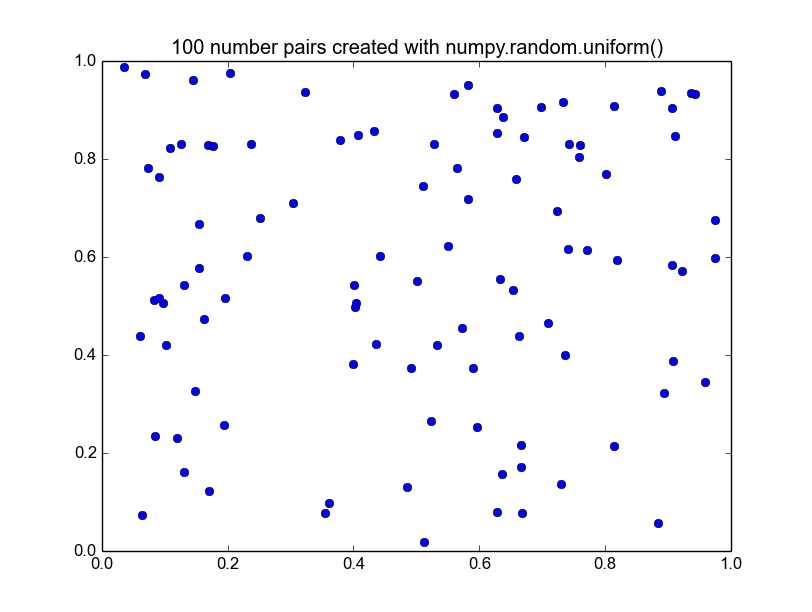
\includegraphics[width=\textwidth]{uniform.png}
        \end{figure}
        \FloatBarrier
    \item $ $
        \begin{figure}[!h]
            \centering
            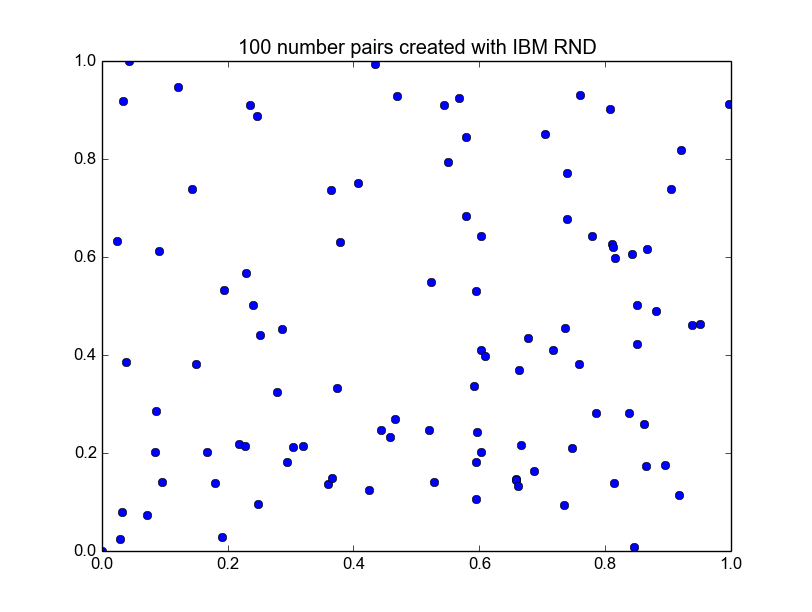
\includegraphics[width=\textwidth]{ibm.png}
        \end{figure}
        \FloatBarrier
        Both random number generators seem to do the same. Though when using
        the same seed for the IBM generator, 983 for the x-axis and 759 for
        the y-axis, we get the same output.

        The code can be seen in \autoref{o22}.
    \item %RANDU wiki explains
        We can show this downside using the numbers that IBM used. $a=65539$,
        $c=0$ and $m=2^{31}$. Every next number is done by multiplying the
        previous one by $65539=2^{16}+3$. So two steps are formed in the
        following way:

        \begin{equation}x_{k+2}=(2^{16}+3) x_{k+1}=(2^{16}+3 )^2 x_{k}\,\end{equation}

        We can expand this in the following way, taking into account that

        $2^{32}\mod2^{31}=0$:
        \begin{equation}x_{k+2}=(2^{32}+6 \cdot2^{16} +9 )x_{k}=[6 \cdot (2^{16}+3)-9]x_{k}\,\end{equation}

        This vorms the following correlation between the three points.

        \begin{equation}x_{k+2}=6(2^{16}+3)x_{k}-9x_{k}=6x_{k+1}-9x_{k}\,\end{equation}
    \item Numpy's random uses the Mersenne Twister pseudo-random number generator.
        The Mersene Twister firstly generates a cache of 32 bit random
        integers. This cache is filled by the seed. Each time one of the
        numbers from the cache is used by shifts, and's, or's and xor's.
        When the end of the cache is reached, it is refilled.
\end{enumerate}
\section{De exponentie\"ele verdeling}

\begin{enumerate}
    \item
        \begin{equation}
        \begin{aligned}
            E[X] &= \frac{1}{\lambda}\\
            Var[X] &= \frac{1}{\lambda^2}
        \end{aligned}
        \end{equation}

    \item $\lambda > 0$ is the parameter of the equation, which is called the
        rateparameter.

    \item Given that maximum likelihood estimate can be written as:
        \begin{equation}
        \begin{aligned}
            \widehat{\lambda} = \frac{1}{\overline{x}}
        \end{aligned}
        \end{equation}

        De $\overline{x}$ can be calculated with all the points $x_1, x_2,
        \cdots x_n$.

        \begin{equation}
        \begin{aligned}
            \overline{x}={1 \over n}\sum_{i=1}^n x_i
        \end{aligned}
        \end{equation}

    \item
        \begin{equation}
        \begin{aligned}
            f_X(x) &= \lambda - \exp^{-\lambda x}\\
            F_X(x) &= 1 - \exp^{-\lambda x}\\
            F^{-1}_X(p) &= -\frac{\log{(1-p)}}{\lambda}\\
        \end{aligned}
        \end{equation}

        See code in \autoref{o3}, and \autoref{fig:exponential}.
        \begin{figure}[h!]
            \centering
            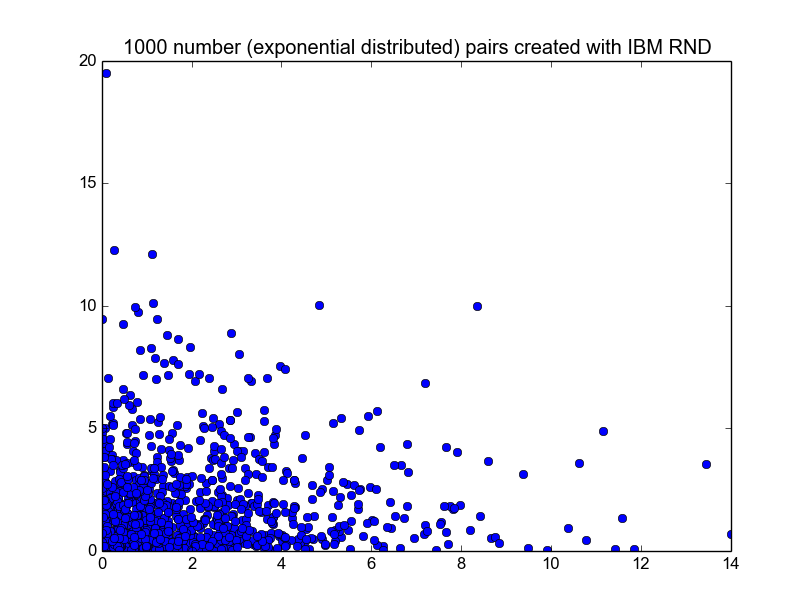
\includegraphics[width=0.8\textwidth]{exponential.png}
            \caption{Exponential distribution function}
            \label{fig:exponential}
        \end{figure}
    \FloatBarrier
    \item See code in \autoref{o3}, and \autoref{fig:histogram}.
        \begin{figure}[h!]
            \centering
            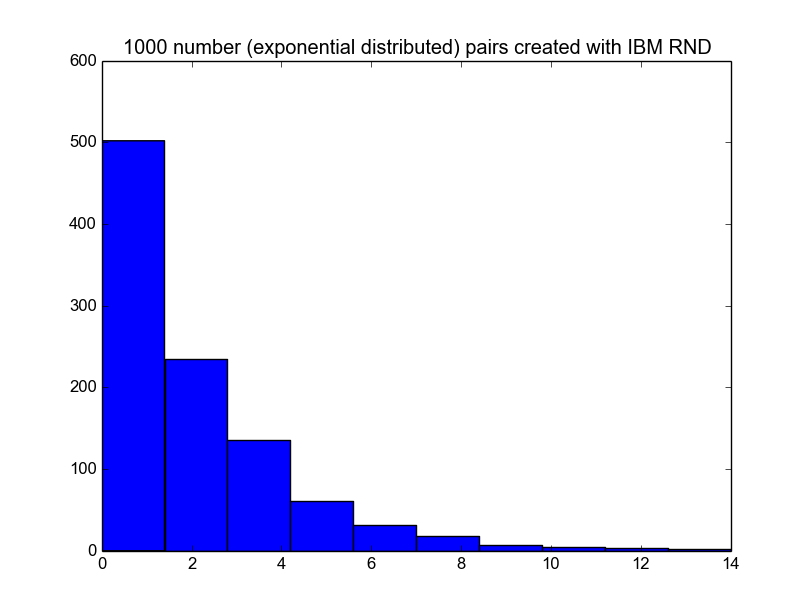
\includegraphics[width=0.8\textwidth]{histogram.png}
            \caption{Histogram of exponential distribution function}
            \label{fig:histogram}
        \end{figure}
    \FloatBarrier
    \item See code in \autoref{o3}, and \autoref{fig:exponential}.

\end{enumerate}

\section{Confidence intervals}

To do statistics on large population, a small subset can be taken. By
calculating a confidence interval of these subsets, the reliability of whole set
can be calculated.

For this assignment there is a set of waiting times. There was a 95\% confidence
interval for the subset, which is of size 50. By calculating the mean ($\mu$) of the
subset and comparing if it falls in the confidence interval 95\% of the mean of
the total set of data, the interval was validated.

The standard deviation ($\sigma$) of the subset is unknown. For that reason the
T-score of the set is calculated. Here $\bar{X}$ is the mean of the subset.

$$ T = \frac{\bar{X} - \mu}{s / \sqrt{n}} $$

To see if the mean of the subset falls within the confidence interval, we have
to check if the T-score value falls within a interval $[-c, +c]$. This $c$ can
be calculated using the inverse cumulative distribution function.

$$ c = F^{-1}_{T(n-1)} (1-\alpha) $$

Because calculating this interval value $c$ is non trivial, a look-up table can
be used. For this experiment we have 50 degree's of freedom and a 95\%
confidence interval is required. Using the look-up table we come to a value of
$c = 2.009$. When $-c \leq T \leq +c$, then the mean of the subset is in the
confidence interval.

While running the code that can be seen in \autoref{confidence}, we came to the
result of 93\%-94\% most of the times. This is in contrast to the 95\% that was
expected.

\appendix
\section{IBM random}
\label{o22}
{\footnotesize\inputminted{python}{o22.py}}

\section{Exponential random}
\label{o3}
{\footnotesize\inputminted{python}{o3.py}}

\section{Confidence Interval}
\label{confidence}
{\footnotesize\inputminted{python}{confidence.py}}
%TODO More discussion?

% =================================== REFERENCES ===================================

%\clearpage
% \bibliographystyle{apalike}
% \bibliography{report}

\end{document}
